\documentclass[a4paper, 12pt, oneside]{book}

\usepackage{titlesec} % Установить отступы для главы равными 0

\titleformat{\chapter}[display]{\normalfont\huge\bfseries}{\chaptertitlename\ \thechapter}{20pt}{\Huge}
\titlespacing*{\chapter}{0pt}{0pt}{0pt} % Установить отступы для главы равными 0

%% подключаем стандарт библиографии
\bibliographystyle{gost71u}

%% for envirovemt "abstract" in class book
\newenvironment{abstract}{}{}
\usepackage{abstract}

%% подключаем преамбулу, в ней содержатся подключение всех необходимых пакетов
%%% Работа с русским языком
\usepackage{cmap}			 % поиск в PDF
\usepackage{mathtext} 		 % русские буквы в формулах
\usepackage[T2A]{fontenc}	 % кодировка
\usepackage[utf8]{inputenc}	 % кодировка исходного текста
\usepackage[russian]{babel}	 % локализация и переносы

%%% Пакеты для работы с математикой
\usepackage{amsmath,amsfonts,amssymb,amsthm,mathtools}
\usepackage{icomma}

%% Номера формул
%\mathtoolsset{showonlyrefs=true} % Показывать номера только у тех формул, на которые есть \eqref{} в тексте.
%\usepackage{leqno}               % Немуреация формул слева

%% Шрифты
\usepackage{euscript}	 % Шрифт Евклид
\usepackage{mathrsfs}    % Красивый матшрифт
% \usepackage{times}       % Times New Roman

%% Поля (геометрия страницы)
\usepackage[left=30mm,right=15mm,top=2cm,bottom=2cm]{geometry}

%% Русские списки
\usepackage{enumitem}
\makeatletter
\AddEnumerateCounter{\asbuk}{\russian@alph}{щ}
\makeatother

%%% Работа с картинками
\usepackage{caption}
\captionsetup{justification=centering} % центрирование подписей к картинкам
\usepackage{graphicx}                  % Для вставки рисунков
\graphicspath{{images/}{images2/}}     % папки с картинками
\setlength\fboxsep{3pt}                % Отступ рамки \fbox{} от рисунка
\setlength\fboxrule{1pt}               % Толщина линий рамки \fbox{}
\usepackage{wrapfig}                   % Обтекание рисунков и таблиц текстом

%%% Работа с таблицами
\usepackage{array,tabularx,tabulary,booktabs} % Дополнительная работа с таблицами
\usepackage{longtable}                        % Длинные таблицы
\usepackage{multirow}                         % Слияние строк в таблице

%% Красная строка
\setlength{\parindent}{2em}

%% Интервалы
\linespread{1.5}
\usepackage{multirow}

%% TikZ
\usepackage{tikz}
\usetikzlibrary{graphs,graphs.standard}

%% Верхний колонтитул
\usepackage{fancyhdr}
\pagestyle{fancy}

%% Перенос знаков в формулах (по Львовскому)
\newcommand*{\hm}[1]{#1\nobreak\discretionary{}{\hbox{$\mathsurround=0pt #1$}}{}}

%% дополнения
\usepackage{float}   % Добавляет возможность работы с командой [H] которая улучшает расположение на странице
\usepackage{gensymb} % Красивые градусы
\usepackage{caption} % Пакет для подписей к рисункам, в частности, для работы caption*

% подключаем hyperref (для ссылок внутри  pdf)
\usepackage[unicode, pdftex]{hyperref}

% убрать пустые новые страницы до каждой новой главы
\usepackage{tocloft}
\setlength{\cftbeforechapskip}{0pt}

\hypersetup{hidelinks}

\let\cleardoublepage\clearpage % % Убираем пустую страницу между главами

\pagestyle{empty} % Убираем верхний колонтитул со всех страниц


% Добавляем нумерацию всех страниц
\usepackage{fancyhdr}
\pagestyle{fancy}
\fancyhf{}
\cfoot{\thepage}

\sloppy %% This can help with overfull \hbox problems, but it may also make the right margin look ragged.

\usepackage[nonumberlist]{glossaries}  %% Подключить список сокращений
\makeglossaries

\usepackage{csquotes} %% Экранировать кавычки ""

\usepackage{algorithm}
\usepackage{algorithmic}

%% Python-код
\usepackage{minted}

%% Ссылки на приложение
\usepackage{hyperref}

%% Абзац
\usepackage{indentfirst}
\setlength{\parindent}{1.25cm}

%% Межстрочный интервал
\usepackage{setspace}
\setstretch{1.5}

%% Times New Roman
%% \usepackage{times}

\setlength{\headheight}{27.11469pt}


\begin{document}
      % \begin{center}
    %% *название института*
    \large\textbf{Министерство образования и науки Российской Федерации \\
    Московский физико-технический институт (государственный университет)} \\
    \vspace{1cm}

    %% *факультет/физтех-школа*
    Физтех-школа прикладной математики и информатики \\

    %% *название базовой кафедры и лаборатории*
    Кафедра дискретной математики \\
    %% Лаборатория (laboratory name)\\

    \vspace{3em}

    Выпускная квалификационная работа бакалавра
\end{center}

\begin{center}
    \vspace{\fill}
    %% *название работы*
    \LARGE{Применение мультиагентного обучения с подкреплением для динамических игр двух лиц}

    \vspace{\fill}
\end{center}


\begin{flushright}
    \textbf{Автор:} \\
    Студент 925 группы \\
    Гимишян Ашот \\
    \vspace{2em}
    \textbf{Научный руководитель:} \\
    кандидат физико-математических наук \\
    Яминов Ринат Ильгизович \\
    \vspace{2em}
    %%\textbf{Научный консультант:} \\
    %%*научная степень* \\
    %%Сергеев Сергей Сергеевич \\
\end{flushright}

\vspace{7em}

\begin{center}
    %% *лого*
    
\includegraphics[width=100 pt]{MIPT_logo.jpg}\\
    Москва \the\year{}
\end{center}

% выключаем отображение номера для этой страницы (титульник)
\thispagestyle{empty}


%\newpage
\setcounter{page}{2}
 %% титульный лист
      \begin{abstract}

    \begin{center}
    \textbf{\large{Применение мультиагентного обучения с подкреплением для динамических игр двух лиц}} \\ 
    \large{Гимишян Ашот} \\ [1 cm]
    \end{center}


\begin{center}
\begin{minipage}{0.8\textwidth}

Работа посвящена исследованию применения мультиагентного обучения с подкреплением в динамических играх двух лиц. В ней представлена модифицированная задача о сделке --- экспериментальная игра из теории игр. Данная игра может быть рассмотрена как модель многих реальных ситуаций, где стороны ведут переговоры о разделе общего ресурса. Она иллюстрирует сложность подобных переговоров и важность учета различных факторов, включая текущую и будущую выгоду, риск, а также влияние на соперника. В ходе исследования была разработана модель искусственного интеллекта, которая путем симуляции двусторонних переговоров эффективно решает данную задачу. Проведенные эксперименты подтвердили практическую значимость модели, отраженную в монотонном возрастании средней награды и уровня согласия между участниками. Полученные результаты могут быть применены для моделирования переговоров и достижения взаимоприемлемых результатов.\\
\end{minipage}
\end{center}

\vspace{20mm}
\textbf{Ключевые слова:} Искусственный интеллект · Машинное обучение · Нейронные сети · Обучение с подкреплением · Теория игр · Динамические игры ·  Модифицированная задача о сделке · Переговоры


    \vfill % используется для заполнения вертикального пространства в документе до конца страницы
    
\end{abstract} %% аннотоция
      \tableofcontents %%содержание
      \printglossary[type=\acronymtype, title=Список сокращений]

      \newacronym{ddpg}{DDPG}{Deep Deterministic Policy Gradient}

\newacronym{maddpg}{MADDPG}{Multi-Agent Deep Deterministic Policy Gradient}

\newacronym{rl}{RL}{Reinforcement Learning}

\newacronym{marl}{MARL}{Multi-Agent Reinforcement Learning}

\newacronym{ppo}{PPO}{Proximal Policy Optimization}

\newacronym{td-learning}{TD-learning}{Temporal-Difference Learning}

\newacronym{wolf}{WoLF}{Win or Learn
Fast}

\newacronym{dcc}{DCC}{Deep Continuous Clustering}

\newacronym{drl}{DRL}{Deep Reinforcement Learning}

\newacronym{dqn}{DQN}{Deep Q-Network}

\newacronym{рн}{РН}{Равновесие Нэша}

\newacronym{инс}{ИНС}{Искусственная нейронная сеть}

\newacronym{ии}{ИИ}{Искусственный интеллект}

\glsaddall
      \chapter{Введение}

\begin{flushright}
\fontsize{10}{12}\selectfont
\textit{Давайте перейдем из эпохи противостояния в эпоху переговоров...}\\
\textit{Ричард Никсон}
\end{flushright}

\label{sec:Chapter0} \index{Chapter0}


В современном мире существует множество задач, которые могут быть решены при помощи технологий искусственного интеллекта. Одной из таких задач является моделирование игр, в которых принимают участие несколько агентов. Это может быть полезным, например, в бизнесе, где агентами могут выступать различные компании. Для них моделирование игр может служить в качестве инструмента прогнозирования рынка, определения стратегий конкуренции и разработки маркетинговой политики. Помимо этого, моделирование игр с несколькими агентами может быть полезным во многих других областях, таких как политика и технологии. В политике моделирование игр может помочь анализировать стратегии и взаимодействия между различными участниками политических процессов. Оно может использоваться для анализа выборов, где различные партии и кандидаты могут выбирать свои стратегии в зависимости от действий своих конкурентов. В технологиях моделирование игр может быть полезно для анализа конкуренции на рынке и разработки новых продуктов и услуг. Компании могут моделировать игры для определения оптимальной стратегии ценообразования на основе поведения конкурентов.


\section{Описание динамических игр двух лиц и мультиагентного обучения с подкреплением}

Пусть у нас есть два игрока, которых мы обозначим как \(A\) и \(B\). Каждый игрок имеет набор возможных стратегий, которые мы обозначим как \(S_A\) и \(S_B\) соответственно. Игрок \(A\) выбирает стратегию \(s_A \in S_A\), а игрок \(B\) выбирает стратегию \(s_B \in S_B\). Выбор стратегии каждым игроком зависит от предыдущих ходов обоих игроков. Выигрыш каждого игрока определяется функцией выигрыша, которую мы обозначим как \(U_A(s_A, s_B)\) для игрока \(A\) и \(U_B(s_A, s_B)\) для игрока \(B\). Эти функции выигрыша зависят от выбранных стратегий обоих игроков. Цель каждого игрока --- выбрать такую последовательность стратегий, которая максимизирует его ожидаемый выигрыш. То есть, игрок \(A\) стремится максимизировать \(U_A(s_A, s_B)\) по всем возможным \(s_A\), а игрок \(B\) стремится максимизировать \(U_B(s_A, s_B)\) по всем возможным \(s_B\).

Что касается MARL, то это подход в машинном обучении при котором агенты обучаются путем взаимодействия друг с другом и с окружающей средой. Каждый агент получает обратную связь от среды в виде награды (англ. reward) или штрафа (англ. penalty) за каждое свое действие. Награда представляет собой меру успеха выполненного действия, а штраф --- меру неудачи.

\begin{figure}[h]
  \centering
  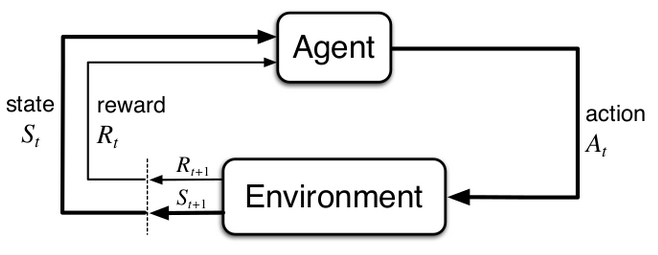
\includegraphics[scale=0.5]{marl.png}
  \caption{Мультиагентное обучение с подкреплением}
\end{figure}

Для моделирования динамических игр с применением обучения с подкреплением и последующего поиска их решений необходимо создать алгоритмы, которые обеспечат взаимодействие агентов в соответствии с заданными правилами и стратегиями. Процесс моделирования можно начать с изучения конфликтной ситуации, которую планируется представить в виде игры и определения предпочтений заинтересованных сторон. В качестве следующего этапа можно рассматривать разработку стратегий и правил. Агенты будут использовать стратегий для достижения своих целей, а правила будут регулировать их поведение. Помимо этого, для эффективного моделирования игр с несколькими агентами необходимо учитывать различные факторы, такие как тип игры, количество и характеристики агентов, возможные исходы при выборе агентами той или иной стратегий. Важно также учитывать возможные изменения в игре и адаптировать стратегии и правила соответствующим образом.


\section{Обоснование выбора темы и актуальность проблемы}

Применение мультиагентного обучения с подкреплением для динамических игр двух лиц является актуальной и перспективной темой для исследования. Приведу несколько аргументов, обосновывающих выбор этой темы и актуальность проблемы:

\begin{enumerate}
    \item Мультиагентное обучение с подкреплением является одним из передовых направлений в области искусственного интеллекта. Изучение применения MARL в динамических играх двух лиц может привести к новым открытиям в разрешении конфликтных ситуации путем переговоров.

    \item В реальных сценариях взаимодействие между агентами играет ключевую роль. Исследование применения мультиагентного обучения с подкреплением в динамических играх двух лиц может помочь разработать новые методы и подходы для эффективного сотрудничества и соперничества между агентами.

    \item Исследование MARL в контексте динамических игр двух лиц может привести к новым применениям в различных отраслях, таких как финансы, экономика, транспорт, робототехника и других. Это может способствовать прогрессу в этих областях и улучшению качества жизни людей.

\end{enumerate}

Мультиагентное обучение с подкреплением является относительно новым направлением исследований в области искусственного интеллекта, которое показало свой потенциал в различных задачах. Мультиагентные системы становятся все более распространенными в различных областях, например, в робототехнике, автономной навигации, финансах, игровой индустрии, бизнесе, политике и других. В таких системах возникает потребность в разработке эффективных методов обучения для агентов, которые позволят им адаптироваться к изменяющимся условиям и достигать высокой производительности в условиях взаимодействия с другими агентами и окружающей средой.


\section{Цель работы и задачи, которые необходимо решить}

Кроме описания различных алгоритмов MARL для решения динамических игр двух лиц, моей целью является разработка новой игры в теории игр --- модифицированной задачи о сделке. Она будет представляться впервые как расширение классической задачи о сделке. В данной игре участники должны соревноваться в некооперативном взаимодействии с целью распределения заданных общих ресурсов между собой. Также собираюсь представить новый подход к распределению ресурсов между участниками, который учитывает влияние участника на переговорный процесс и на основе этого подхода разработать модель искусственного интеллекта, способную решить модифицированную задачу о сделке. Модель будет обучена для поиска оптимальных стратегий и обеспечения эффективной коммуникации между участниками, а также для адаптации к изменяющимся условиям и поведению всех участников.

С помощью математики и искусственного интеллекта хочется создать прикладной инструмент для решения следующих проблем:

\begin{enumerate}
    \item Формализация завершенных конфликтных ситуации, соответствующих описанию данной игры, с целью выяснения на каком этапе стороны не смогли достичь соглашения и каковы были их убытки.

    \item Формализация действующих конфликтных взаимодействий на ранних этапах развития и предложение оптимальных исходов разрешающих такие ситуаций. Доказательство того, что искусственному интеллекту можно доверять разрешение конфликтов.

    \item Моделирование взаимодействии, которые потенциально могут вызвать конфликты в реальной жизни. Учитывая влияние участников на обстановку, их силы, интересы и временной фактор, предложить возможные варианты решении.
\end{enumerate}

Во вступительной части \textbf{первой главы} представлена ознакомительная информация. Глава включает определения MARL и динамических игр. Далее изложены аргументы мотивирующие выбор темы и её актуальность в современных условиях. В завершении главы кратко описывается проблема, которую необходимо решить, и формулируются общие цели дипломной работы.

Во \textbf{второй главе} проведен анализ основных публикаций, посвященных теме игр двух лиц и мультиагентного обучения с подкреплением. Здесь рассмотрены ключевые исследования, описывающие различные подходы и техники, которые сформировали основу современных методов в этой области. Кроме того, дано формальное описание задачи о сделке. Дополнительно сделан подробный обзор существующих подходов к решению этой задачи..

В \textbf{третьей главе} дана формулировка модифицированной задачи о сделке. Там же обоснована необходимость перехода от классической к модифицированной версии задачи о сделке. В заключительной части главы описана мотивация применения методов машинного обучения для решения данной задачи.

\textbf{Четвертая глава} посвящена подробному описанию и сравнению выбранных алгоритмов мультиагентного обучения с подкреплением и их применению к модифицированной задаче о сделке. Обсуждается выбор алгоритмов, процесс обучения и оптимизации, а также обосновывается их применимость для решения данной задачи.

\textbf{Пятая глава} представляет результаты экспериментов, проведенных для оценки эффективности разработанной модели в решении модифицированной задачи о сделке. Здесь описывается среда, в которой проводились эксперименты, и набор данных, использованный для обучения и оценки модели.

Результаты работы обсуждаются в заключительной, \textbf{шестой главе}. В ней также раскрывается прикладная значимость и ценность проведенного исследования. К тому же, данная глава содержит рекомендации по дальнейшему развитию и расширению сферы применения полученных результатов. %% Введение
      \chapter{Обзор литературы}
\label{sec:Chapter1} \index{Chapter1}


В этой главе представлю итоги анализа наиболее влиятельных и значимых результатов, связанных с играми двух лиц и мультиагентным обучением с подкреплением. Моя цель состоит в том, чтобы представить вам ключевые исследования, которые сформировали основные направления и подходы в данной области. Я уделю внимание на разнообразие методов, применяемых учеными для решения задач и преодоления сложностей, связанных с мультиагентными системами. Этот обзор позволит лучше понять существующие подходы и их взаимосвязь, а также определить перспективы развития данной области науки. Кроме того, я дам формальное описание классической задачи о сделке. Далее в работе будет представлено формальное описание модифицированной задачи о сделке, поэтому важно уже сейчас ознакомиться с классической версией этой экспериментальной игры, чтобы понять различия.


\section{Краткий обзор основных публикаций по теме игр двух лиц и мультиагентного обучения с подкреплением}

В своей статье \cite{nash50} Джон Нэш предложил понятие РН, которое стало фундаментальным в теории игр. РН представляет собой набор стратегий в игре для двух и более игроков, в котором ни один участник не может увеличить выигрыш, изменив свою стратегию, если другие участники своих стратегий не меняют. Нэш доказал существование такого равновесия в смешанных стратегиях в любой конечной игре.

Здесь \cite{littman94} Майкл Литтман предложил марковские игры (стохастические игры) в качестве основы для мультиагентного обучения с подкреплением. Марковские игры являются расширением марковских процессов принятия решений, учитывающих действия нескольких агентов. Автор применил этот подход к кооперативным и конкурентным задачам, демонстрируя его применимость в различных сценариях.

Джералд Тесауро представил TD-Gammon в \cite{tesauro95}. Это программа для игры в нарды, использующую \textbf{TD-обучение} (обучение с подкреплением на основе временной разницы). TD-Gammon стал одним из первых успешных примеров применения обучения с подкреплением в играх и продемонстрировал возможность разработки высокопроизводительных агентов без явных знании. Модель была обучена без знания правил и стратегий игры, а только на основе информации об успехе или неудаче своих ходов. Такой подход показал возможность создания высокопроизводительных агентов без предварительного знания о специфике проблемы, что стало важным шагом в развитии обучения с подкреплением и искусственного интеллекта в целом.

В своей работе \cite{bowling02} Боулинг и Велозо представили алгоритм для мультиагентного обучения с использованием переменной скорости обучения (\textbf{WoLF}). Алгоритм меняет скорость обучения в зависимости от оценки эффективности текущей стратегии агента. Этот подход позволяет агентам лучше адаптироваться к изменяющимся ситуациям в мультиагентных средах.

Обзор \cite{busoniu08} представляет собой широкий анализ методов мультиагентного обучения с подкреплением, включая их теоретические основы, алгоритмы и применение в различных областях. Авторы обсуждают как кооперативные, так и конкурентные сценарии, а также коммуникацию между агентами. Они также рассматривают вопросы сходимости, обучения и адаптации в мультиагентных системах.

В статье \cite{foerster16} авторы представили метод глубокого мультиагентного обучения с подкреплением, который позволяет агентам обучаться совместной кооперативной коммуникации с использованием \textbf{DCC}. Это подход к обучению, в котором агенты обмениваются информацией и настраивают свои стратегии на основе обратной связи других агентов, что позволяет им успешно решать сложные задачи, требующие кооперации.

В работе \cite{lowe17} авторы представили алгоритм \textbf{MADDPG}, который является расширением алгоритма DDPG для мультиагентных сред. MADDPG основан на актор-критике, где каждый агент имеет собственные актор и критик, обучаемые независимо. Он позволяет агентам совместно обучаться в смешанных средах, где они могут взаимодействовать как кооперативно, так и конкурентно. Этот алгоритм продемонстрировал успех в решении сложных мультиагентных задач, таких как управление движением и командные игры.

Статья \cite{legleau20} исследует применение мультиагентного обучения с подкреплением, используя \textbf{Q-обучение} в ультиматумной игре. Авторы применяют Q-обучение для обучения агентов и используют $\epsilon$-жадную стратегию, позволяющую агентам исследовать и эксплуатировать среду. Цель исследования состоит в том, чтобы анализировать и сравнивать различные стратегии агентов, чтобы определить наиболее эффективные подходы в ультиматумной игре.

В статье \cite{chang20} автор применяет глубокое обучение с подкреплением (\textbf{DRL}) для обучения агентов в мультиагентных переговорах. Это исследование направлено на поиск оптимальных стратегий и результатов в сложных переговорах, где участники обсуждают несколько вопросов. Агенты, представленные глубокими нейронными сетями, учатся оптимальной стратегии, основываясь на взаимодействии с окружающей средой и получении подкрепления за свои действия.

\cite{schulman2017ppo} --- статья, в которой представлен метод \textbf{PPO}. Данный метод призван решить некоторые проблемы с обучением с подкреплением, связанные с нестабильностью и большим временем обучения. PPO является методом оптимизации политики, который использует технику, известную как обрезка (англ. clipping), чтобы ограничить обновления политики в каждой итерации оптимизации.

Работа \cite{mnih2013dqn} является одной из первых, в которой обсуждается сочетание глубокого обучения и обучения с подкреплением. Авторы представили алгоритм, который они назвали \textbf{DQN}. Он сочетает Q-обучение, метод обучения с подкреплением, с глубокими нейронными сетями.

В \ref{sec:Chapter3}-ой главе подробно описаны некоторые из упомянутых алгоритмов. Там же выбран алгоритм для решения модифицированной задачи о сделке. Подбор подходящего алгоритма сопровождается подробными комментариями.


\section{Описание существующих подходов к решению задачи о сделке и их ограничения}

\subsection{Задача о сделке}

Задача о сделке --- экспериментальная экономическая игра двух лиц в теории игр, которая моделирует процесс двусторонних переговоров. В этой игре участники должны договориться о распределении конечного объема общих ресурсов. На практике такое взаимодействие возникает в случае, когда торговля может принести прибыль, например, одна из сторон ценит ресурсы меньше. Более того, для моделирования переговоров и анализа такой проблемы необходимо отсутствие установленных ценовых норм на рынке.

Итак, на столе переговоров денежная сумма $M$ --- прибыль от торговли. Игроки ходят поочередно. Суть игры заключается в том, что первый игрок предлагает распределить $M$ в пропорциях $(x, M - x)$. Такой дележ реализуется при наличии согласия второго игрока. В результате его реализации первый получает $x$, второй --- $M - x$. Если игроки не приходят к соглашению, то каждый получает свою часть заранее фиксированного исхода $(a, b)$. Первый получает $a$, второй --- $b$. Следует отметить, что в подавляющем большинстве реальных случаев $a = b = 0$. Предполагается, что $a + b < M$.

Формально задачу о сделке можно представить в виде кортежа $(N, X, u)$, где

\begin{itemize}

\item $N$ --- множество игроков. В этой игре $|N| = 2$, то есть участвуют два игрока, которые обычно называются Игрок 1 и Игрок 2.

\item $X$ --- пространство исходов. $X = \left\{ (x, y) \in \mathbb{R}_{\geq 0}^2: x + y = M \right\}$. Оно является непрерывным и линейным. В этой работе мы не будет нормировать его, то есть не будем рассматривать $\frac{x}{M} + \frac{y}{M} = 1$ вместо $x + y = M$.

\item $u = (u_1, u_2)$ --- пара функций полезности, которая представляет предпочтения каждого игрока относительно результатов в $X$. Функция полезности $u_i: X \rightarrow \mathbb{R}_{\geq 0}$ представляет предпочтения Игрока $i$.

\end{itemize}

Цель игры --- добиться соглашения между участниками о том, как распределить ресурсы. Из-за разногласий в предпочтениях по результатам в $X$ можно наблюдать конфликт интересов. Задача о сделке моделирует этот конфликт как игру стратегического взаимодействия, где каждый игрок пытается договориться о сделке, которая максимизирует его собственную функцию полезности.

Данная задача является важной для понимания того, как агенты принимают решения в условиях конкуренции и ограниченности ресурсов. Ее формализация помогает лучше понять проблемы ведения переговоров в различных экономических ситуациях. Были разработаны различные методы решения этой игры. Одним из распространенных способов решения является решение Нэша. Оно представляет собой набор результатов, которые оба игрока предпочитают любому альтернативному результату. Решение Нэша основано на концепции справедливости, которая предполагает, что оба игрока имеют равную силу в переговорах.\\


\subsection{Решение двухходовой задачи о сделке}

Игра \enquote{Ультиматум} --- двухходовая задача о сделке, описанная выше, является простейшим вариантом задачи о сделке, которая имеет следующее решение: второй игрок примет предложение $(x, M - x)$, если $ M - x \geq b $. Предположим, $ x = M - b $. Если первый игрок изменит свою стратегию с целью максимизации собственного выигрыша, то второму будет выгодно отказать. Кроме того, заметим, что при получении предложения $(M - b, b)$ любая стратегия (принять или отклонить) второго игрока приносит прибыль не больше $b$. Следовательно, исход $(M - b, b)$ является РН. Здесь очевидным недостатком является наличие равновесия $(M, 0)$ при $b = 0$. Таким образом, в реальной ситуации первый агент может оставить себе всю денежную сумму $M$. Формально это будет считаться равновесием. 


\subsection{Переговоры о цене недвижимости}
Пример из реальной жизни:

\begin{itemize}

    \item Продавец не готов продать свою недвижимость меньше $4{,}500{,}000$ рублей.
    
    \item Покупатель готов платить не больше $5{,}000{,}000$ рублей.
        
    \item $M = 5{,}000{,}000-4{,}500{,}000 = 500{,}000, a = b = 0$.
    
    \item Предположим продавец ходит первым и обладает совершенной информацией. Он знает, что покупатель отклонит любое предложение $> 5{,}000{,}000$ и примет любое $\leq 5{,}000{,}000$.
    
    \item Продавец максимизирует свою прибыль предлагая цену равную $5{,}000{,}000$ или $x = 500{,}000$. Покупатель принимает, ведь $M - x \geq b$.
    
    \item Продавец получает $500{,}000$, то есть всю денежную сумму $M$, покупатель --- 0.
    
\end{itemize}

\begin{figure}[h]
  \centering
  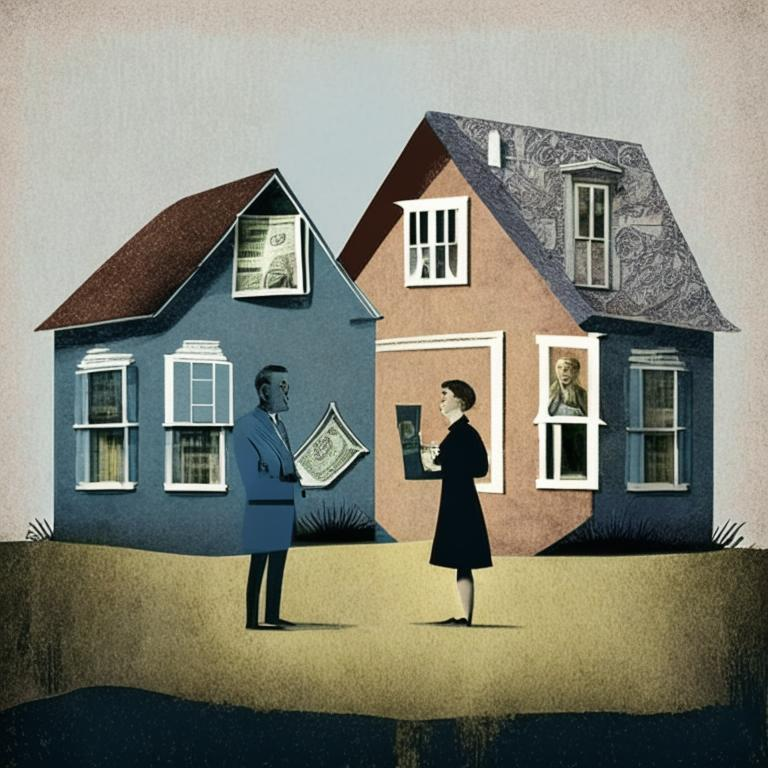
\includegraphics[scale=0.2]{simple_bargaining_game_house.jpg}
  \caption{Переговоры о стоимости недвижимости}
\end{figure}

\textbf{Вывод:} покупатель не должен заранее объявить максимальную сумму, которую готов платить за недвижимость. Эту информацию продавец может использовать против него. В том числе из этих соображений я буду рассматривать игру с неполной информацией.


\subsection{Двухходовка с сокращением прибыли}

Предположим, что $M=12$, $\delta=\frac{1}{3}$ — коэффициент дисконтирования. Обратите внимание, что во втором раунде $M=4$. Игрок $2$ знает, что может получить $3.99$ в раунде $2$, поскольку Игрок $1$ предпочтет $0.01$ ничему и примет дележ $(0.01, 3.99)$. Это следует из предположения что игроки ориентированы на будущее, рациональны и максимизируют свой выигрыш. Учитывая это, Игрок $1$ должен предложить Игроку $2$ $4.00 > 3.99$ в первом раунде, оставив себе $12 - 4 = 8$. Поскольку Игрок $2$ понимает, что ни в каком исходе не может получить больше $4.00$, он примет дележ $(8.00, 4.00)$. Предложение Игрока $1$ отдать $4.00$ Игроку $2$ в первом раунде равно сумме ставки в начале финального раунда, умноженной на коэффициент дисконтирования, $\delta \cdot M$. Такое предложение приведет к равновесию. Это обобщается на любую задачу о сделке с $n$ раундами, где $2 < n < \infty$.

Этот пример показывает, что в игровой ситуации, где участники направлены на долгосрочные результаты, действуют рационально и стараются максимизировать свои выигрыши, возможно достижение РН, которое обеспечивает оптимальные исходы. В данном случае, для достижения РН Игрок $1$ в первом раунде предлагает Игроку $2$ условия, которые выгодны обоим, чтобы Игрок $2$ принял предложение и не стремился получить больше в следующем раунде.

\textbf{Вывод:} в задачах о сделке можно достичь РН, которое приводит к эффективному результату, если участники сделки обладают достаточной информацией о возможных исходах, являются рациональными и ориентированы на будущее. Однако, если эти условия не выполняются, могут возникнуть проблемы координации и нежелательные исходы.


\subsection{Переговоры о цене недвижимости (продолжение)}

\begin{itemize}

\item Минимальная стоимость, по которой продавец продаст свою недвижимость составляет $15{,}000{,}000$ рублей, а максимальная цена, которую покупатель готов заплатить --- $16{,}000{,}000$ рублей. Следовательно, $M = 1{,}000{,}000$ рублей.

\item Оба игрока имеют одинаковый коэффициент дисконтирования $\delta=0.8$.

\item Процесс переговоров ограничен двумя раундами. Это обусловлено тем, что продавец обязан продать недвижимость до определенного срока (возможно, для покупки другой недвижимости), а покупателю, в свою очередь, нужно приобрести эту недвижимость до определенной даты.

\item В первом раунде переговоров предложение выдвигает покупатель, а во втором раунде --- продавец.

\item Следует применить метод обратной индукции, начав анализ с последнего, второго раунда переговоров и двигаться в обратном направлении для поиска оптимальной последовательности действии.

\item С точки зрения сегодняшнего дня потенциальный суммарный выигрыш от сделки во втором раунде составляет $\delta \cdot M$. На этом этапе на продавце лежит обязанность предложить контрпредложение.

\item В заключительном раунде продавец предложит оставить себе $\delta \cdot M$, предоставляя покупателю возможность принять или отклонить это предложение. На этом этапе покупателю нет разницы между принятием или отклонением предложения. В обоих случаях его выигрыш равен $0$.

\item Осознавая это, покупатель в первом раунде должен предложить продавцу $\delta \cdot M$. Продавец, будучи равнодушным между ожиданием и немедленным принятием, принимает данное предложение.

\item В нашем примере, где $\delta = 0.8$ и $M = 1{,}000{,}000$, покупатель предлагает продавцу $0.8 \cdot M$ или $800{,}000$, оставляя себе $200{,}000$. Таким образом, стоимость недвижимости составляет $15{,}000{,}000 + 800{,}000 = 15{,}800{,}000$.

\end{itemize}


\subsection{Анализ бесконечно повторяющихся игр}

\begin{itemize}
\item Теперь предположим, что количество переговорных раундов не ограничено. Переговоры могут продолжаться бесконечно.

\item Если покупатель делает предложение первым, то сумма $x(1) \cdot M$, которую он намерен оставить себе в первом раунде, должна гарантировать продавцу приемлемую выгоду. Эта выгода должна быть не меньше той, которую продавец может получить в следующем раунде, если отклонит текущее предложение и предложит забрать $y(2) \cdot M$. Иными словами, в первом раунде продавец должен получить сумму, эквивалентную $\delta \cdot y(2) \cdot M$.

\item Покупатель предлагает продавцу $(1 - x) M = \delta y M$, и таким образом, $x = 1 - \delta y$.

\item Аналогичным образом, продавец должен предложить покупателю $(1 - y) M = \delta x M$. Следовательно, $y = 1 - \delta x$.

\item Получаем систему уравнений:
\begin{equation}
\begin{cases}
    x &= 1 - \delta (1 - \delta x), \\
    y &= 1 - \delta (1 - \delta y).
\end{cases}
\end{equation}

\item $x = y = \frac{1-\delta}{1-\delta^2}$. Обратите внимание, что $x+y > 1$.

\item $x$ и $y$ обозначают суммы, которые получают покупатель и продавец соответственно, если они делают первое предложение в первом раунде.

\end{itemize}


\subsection*{Практические выводы}

\begin{enumerate}

\item В реальной жизни стороны переговоров не знают коэффициенты дисконтирования друг друга или их относительные уровни терпения, но могут пытаться угадать эти значения.

\item Нужно подать сигнал о том, что вы терпеливы, даже если на самом деле нет. Например, не отвечать контрпредложениями сразу же.

\item Более терпеливый игрок получает большую часть суммы $M$, которая находится на столе переговоров.

\end{enumerate} %% Постановка задачи
      \input{parts/Chapter2.tex} %% Обзор существующих решений
      \input{parts/Chapter3.tex} %% Исследование и построение решения задачи
      \input{parts/Chapter4.tex} %% Описание практической части
      \input{parts/Chapter5.tex} %% Заключение

    %% Don't change the following lines
      \nocite{*}
      \bibliography{references}

    %% в зависимости от надобности подключаем раздел "Приложениие"
    % \newpage
      \chapter{Приложение}
\label{sec:Chapter6} \index{Chapter6}

\section{Реализация классов ActorNetwork и CriticNetwork на Python}

\label{sec:networks}

\begin{minted}{python}
class ActorNetwork(nn.Module):
    def __init__(self, state_dim, action_dim, hidden_dim):
        """
        Инициализация акторной сети.
        Args:
        - state_dim (int): Размерность состояния.
        - action_dim (int): Размерность действия.
        - hidden_dim (int): Размерность скрытых слоев в сети.
        """
        super(ActorNetwork, self).__init__()
        self.fc1 = nn.Linear(state_dim, hidden_dim)
        self.fc2 = nn.Linear(hidden_dim, hidden_dim)
        self.fc3 = nn.Linear(hidden_dim, action_dim)
        self.relu = nn.ReLU()
        self.tanh = nn.Tanh()

    def forward(self, state):
        """
        Прямой проход через акторную сеть.
        Args:
        - state (torch.Tensor): Входное состояние.

        Returns:
        - action (torch.Tensor): Выходное действие.
        """
        x = self.relu(self.fc1(state))
        x = self.relu(self.fc2(x))
        x = self.tanh(self.fc3(x))
        return x

    
class CriticNetwork(nn.Module):
    def __init__(self, state_dim, action_dim, hidden_dim):
        """
        Инициализация критической сети.
        Args:
        - state_dim (int): Размерность состояния.
        - action_dim (int): Размерность действия.
        - hidden_dim (int): Размерность скрытых слоев в сети.
        """
        super(CriticNetwork, self).__init__()
        self.fc1 = nn.Linear(state_dim + action_dim, hidden_dim)
        self.fc2 = nn.Linear(hidden_dim, hidden_dim)
        self.fc3 = nn.Linear(hidden_dim, 1)
        self.relu = nn.ReLU()

    def forward(self, state, action):
        """
        Прямой проход через критическую сеть.
        Args:
        - state (torch.Tensor): Входное состояние.
        - action (torch.Tensor): Входное действие.

        Returns:
        - q_value (torch.Tensor): Выходное значение Q-функции.
        """
        x = torch.cat([state, action], dim=-1)
        x = self.relu(self.fc1(x))
        x = self.relu(self.fc2(x))
        x = self.fc3(x)
        return x 

\end{minted}


\section{Функция main() для инициализации параметров и запуска обучения}

\begin{minted}{python}
def main():
    sum_of_money = 100.0  # Общая сумма денег
    a = 1 # Первый агент получит a, если итоговое соглашение не будет достигнуто
    b = 1 # Второй агент получит b, если итоговое соглашение не будет достигнуто
    num_agents = 2  # Количество агентов в модифицированной задаче о сделке
    discount_factor = 0.99  # Коэффициент дисконтирования
    epsilon_1 = 0.75 # Сила первого агента
    epsilon_2 = 0.74 # Сила второго агента
    
    env = NegotiationEnvironment(sum_of_money, a, b, discount_factor, epsilon_1,
    epsilon_2)  # Инициализация среды переговоров
    
    # Инициализация агентов
    agent1 = MADDPGAgent(agent_id=0, state_dim=env.state_dim,
    action_dim=env.action_dim, hidden_dim=128)
    agent2 = MADDPGAgent(agent_id=1, state_dim=env.state_dim,
    action_dim=env.action_dim, hidden_dim=128)
    agents = [agent1, agent2]  # Список агентов
    
    batch_size = 64     # Размер пакета для обучения
    num_episodes = 1000 # Количество эпизодов обучения

    # Запуск обучения
    train_maddpg(env, agents, num_episodes, batch_size)
\end{minted}
\end{document}